\documentclass{article}
\usepackage[table]{xcolor}
\usepackage{array}

\newcolumntype{P}[1]{>{\raggedright\vrule height4ex width 0pt}p{#1}<{\vrule depth 2.5ex width 0pt}}


\usepackage{cite}
\usepackage[unicode,pdftex]{hyperref}
\usepackage{enumerate}
\usepackage{setspace}
\usepackage{pslatex} 
\usepackage{fancyhdr}
\usepackage{float}
\usepackage{amsmath}
\usepackage{titling}
\usepackage{indentfirst}
\usepackage{graphicx}
\usepackage{wrapfig}
\usepackage{amsmath}
\usepackage{xstring}
\usepackage{tikz}
\usetikzlibrary{fit, calc}
\pagestyle{empty} 
\usepackage{array}


% \geometry{left=2.5cm, right=2.5cm, top=1.4cm, bottom=2.4cm}
\usepackage[a4paper,top=3cm,bottom=2cm,left=3cm,right=3cm,marginparwidth=1in, margin=1in]{geometry}


\title{Frequency Regularization: Efficient Neural Network Compression for Mobile Device Deployment}
\author{Wenhao You(wyou1@ualberta.ca)\\Leo Chang(chewei@ualberta.ca)}
\date{}

\newcommand{\reffig}[1]{Fig. \ref{#1}}
\newcommand{\refsec}[1]{Section \ref{#1}}
% \newcommand{\refeq}[1]{Eq. \ref{#1}}
\newcommand{\reftab}[1]{Table \ref{#1}}

\fancyhead{}
%\lhead{\scriptsize Chenqiu Zhao}
\rhead{\scriptsize research Proposal}

\renewcommand{\headrulewidth}{0pt}
\renewcommand{\normalsize}{\fontsize{12pt}{\baselineskip}\selectfont}


\begin{document}
	\maketitle
	%\vspace{-90pt}
	
	\section{Abstract}

In general, neural networks require high-specification hardware because of their complexity. However, in daily life, people have the requirements for running neural network applications on their own mobile devices but have limited hardware. Even the researchers have to use the computer in their lab instead of running the pre-trained models by using mobile devices. In this proposal, we will focus on how to implement a simple and creative compression algorithm called Frequency Regularization (FR)~\cite{zhao2023frequency}, which is to compress a basic neural network on Android mobile devices. We also discuss another three existing methods to achieve the goal: upgrade hardware~\cite{akusok2019metal}, implement NestDNN~\cite{fang2018nestdnn}, and implement ``One-shot Whole Network Compression"~\cite{kim2016compression}. The reason we did not choose to upgrade mobile hardware is that it is difficult to achieve in a short course time. Moreover, the other two compression algorithms are more difficult to implement and not as efficient as FR. Hence, it is the reason we chose FR to do further research.

% \textbf{Index Terms}: Compressed Neural Networks, Frequency Regularization, Limited Hardware Devices, Mobile Devices, UNet (?)


	\section{Introduction}
	
Neural networks have been implemented in many applications and performed great results. However, these neural networks are usually implemented on high-specification hardware such as computers. The reason is because there are many parameters in different neural networks. The more parameters in the neural networks, the more storage and internet transmission rates are occupied. In this research, we try to look for a method that can make the neural networks run on a limited hardware device, such as a mobile device. Although mobile devices have more enhanced hardware nowadays, because of their limited size, the efficacy is still not as powerful as the computers. There are several benefits of running the neural networks on limited hardware devices, specifically, mobile devices. The most important parts are the privacy~\cite{wang2018privacy} and the data security. Processing data on-device ensures that personal information does not need to be uploaded or transmitted to the cloud servers, which enhances privacy~\cite{wang2018privacy}. 

% in the privacy section, add the citation of this paper: https://arxiv.org/pdf/1809.03428.pdf

Running neural networks on mobile devices can also bring other advantages. If we can implement the neural network models directly on mobile devices, it can reduce our dependence on the internet connection to some extent. Since mobile devices play a significant role in our daily lives, the procedures can be accessed easily. Moreover, for some applications that need real-time feedback, such as object recognition and image segmentation, neural networks on mobile devices can also make the process faster to improve user experience. The most important part of modern life is that we can keep the data processing and inference in the internal system of mobile devices rather than sending it to a remote server, which can increase the processing speed.

The new method, Frequency regularization (FR)~\cite{zhao2023frequency}, is based on the frequency domain to compress the neural network. It is divided into two steps: dynamic tail-truncation and inverse discrete cosine transform (IDCT). The main idea of this method is that some of the neural network parameters may be redundant in their representation. The algorithm focuses on using the frequency domain transform for network regularization to restrict information redundancy during the training process and introduce FR as shown in Fig.~\ref{idct}. Therefore, the redundant part can be removed without any side effect on the performance of the network.

\begin{wrapfigure}{l}{0.5\textwidth}
	\vspace{-15pt}    % 对应高度1
	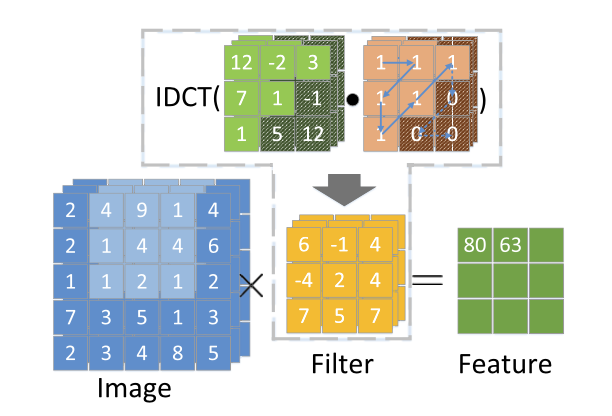
\includegraphics[width=0.5\textwidth]{figure/idct.png}\\
	\vspace{-15pt}    % 对应高度2
	\caption{Illustration of the proposed frequency regularization. The tail elements of tensors in the frequency domain are truncated first, then input into the inverse of the discrete cosine transform to reconstruct the spatial tensor for learning features~\cite{zhao2023frequency}.}
	\label{idct}
	\vspace{-15pt}    % 对应高度3
\end{wrapfigure}


% in presentation
% To implement neural networks on mobile devices, we need to discuss the limitations of hardware and its characteristics. Many popular deep learning libraries, such as PyTorch and TensorFlow, are not complete and perfect to implement directly on mobile devices. Thus, we need to edit some configurations to optimize for mobile devices. Using the implementation, we can convert our standard neural network models into a lighter version that fits the mobile devices' hardware better. Moreover, beyond this idea, we can also consider improving the hardware parts such as creating special neural network processors for the mobile. 

% check the text below
The known shortcoming of this algorithm is the training speed compared to other training methods, which is slower. To apply Frequency Regularization on the neural network and implement it on mobile devices, we will encounter two challenges. (i) The PyTorch library may not be capable of this new algorithm. Therefore, we need to adjust some parameters. (ii) The mobile hardware limitation that can restrict the algorithm to run. 

From the above paper mentioned, Frequency Regularization performs a better compression and works on most general neural networks ~\cite{zhao2023frequency}. Combining the best of our knowledge, we believe this research contributes as the first implementation of applying Frequency Regularization to neural networks but on limited hardware devices, specifically, mobile devices.
% end check

% we need to find the short come of this algorithm
% we need to provide a reference about enhancing privacy
% main contribution 


In conclusion, this paper explores a simple, efficient, and creative method to run a large neural network on mobile devices based on the Frequency regularization algorithm. Our purpose is not only to accomplish this implementation, we want to ensure the performance is similar to the result running on high-specification hardware such as computers. We hope to provide a fast and secure neural network application experience on mobile devices.


\section{Brief Summary of Existing Work}

We cover the methods for implementing neural networks on the mobile over five sections. In Section~\ref{upgrade_hardware}, upgrading hardware on mobile devices and which parts are introduced. At the algorithm level, there is method called Extreme Learning Machine (ELM)~\cite{akusok2019metal}, which assigns hidden layer weights randomly. Section~\ref{elm} shows the biref introduction of ELM. What's more, there is an algorithm called NestDNN~\cite{fang2018nestdnn} based on the dynamics or runtime resources to enable resource-aware multi-tenant on-device deep learning for mobile vision systems as shown in Section~\ref{nestdnn}. Moreover, there is an algorithm called “one-shot whole network compression”~\cite{kim2016compression} to compress convolutional neural networks (CNNs) for mobile deployment as shown in Section~\ref{oneshot}. There is also an algorithm named Frequency Regularization that helps compress the neural network by using the idea of reducing the redundancy information during the training process. The general steps are as shown and introduced in Section~\ref{fr}.

\subsection{Upgrade Hardware}\label{upgrade_hardware}
Hardware accelerators such as the digital signal processors offer solutions to overcome these challenges. Many manufacturers have already produced better hardware. For example, Apple presented the Metal Performance Shaders with the support of CNNs accelerated by GPU. This is a solution built on top of the Metal API and allows custom operations. Since there is an experiment~\cite{akusok2019metal} that confirmed the feasibility of Big Data analysis on modern mobile devices. Moreover, the hardware on Android devices is upgraded by four main companies, such as Qualcomm, HiSilicon, MediaTek, and Samsung~\cite{Andrey2019Aibenchmark}, which can work with neural networks as well.

\subsection{Algorithm Extreme Learning Machine (ELM)}\label{elm}
The Extreme Learning Machine (ELM) is able to allocate the weight of the hidden layers randomly.  And it can generate linear output layer as well. Compared with the traditional neural networks, ELM provides faster training speed and high efficiency. The main idea of ELM is to generate the random hidden nodes, in order to avoid backpropagation. Its advantages are the simplicity, the efficiency, and the fast training speed. However, the biggest disadvantage of ELM is the sensitivity to the number of hidden nodes. In the experiement~\cite{akusok2019metal}, ELM was proved to achieve the same performance with other deep learning models in many tasks. Moreover, ELM is easy to optimize since it has simple structure.

\subsection{Algorithm NestDNN}\label{nestdnn}
\begin{figure}[htbp]
	\centering
	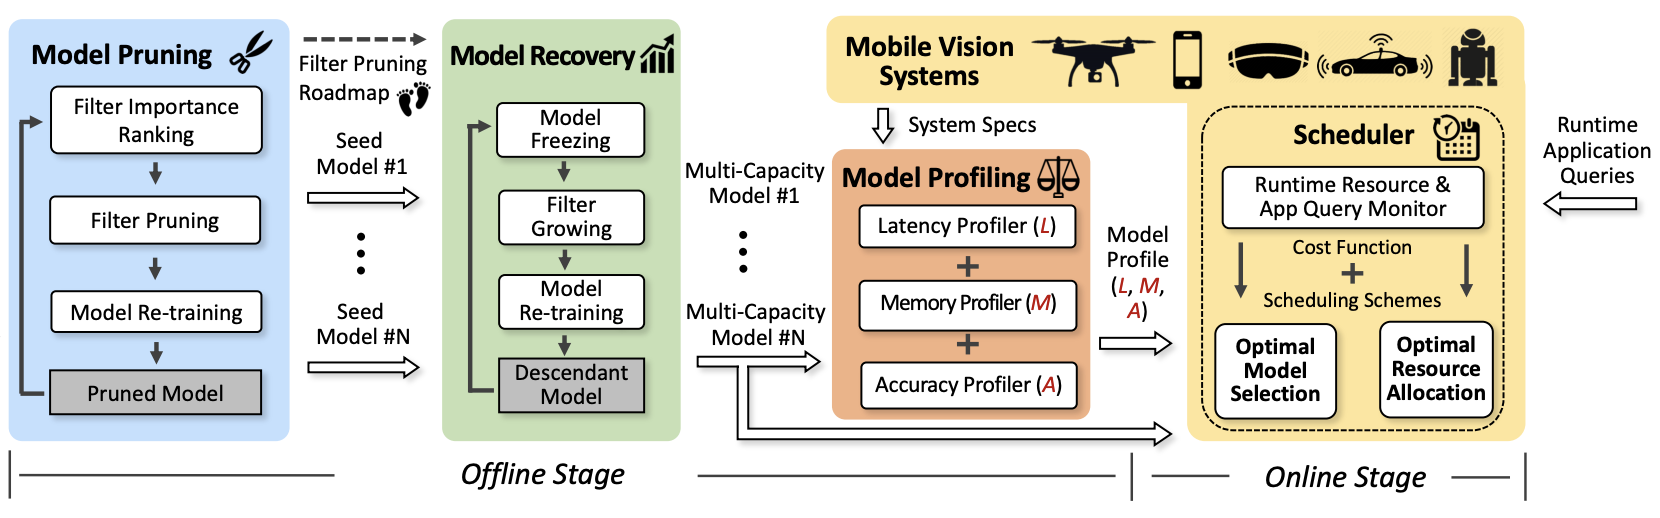
\includegraphics[width=1\linewidth]{figure/nestdnn_arch.png}
	\caption{NestDNN architecture~\cite{fang2018nestdnn}.}
	\label{nestdnn_arch}
\end{figure}

NestDNN is a framework that takes the dynamics of runtime resources into account to enable resource-aware multi-tenant on-device deep learning for mobile vision systems. NestDNN enables each deep learning model to offer flexible resource-accuracy trade-offs~\cite{fang2018nestdnn}. Fig.~\ref{nestdnn_arch} illustrates the architecture of NestDNN in detail, which is split into an offline stage and an online stage. The offline stage consists of three phases: model pruning, model recovery, and model profiling~\cite{fang2018nestdnn}. Table~\ref{nest-table} illustrates the five models involved in NestDNN.

\begin{table}[htbp]
	\centering
	\caption{Five terminologies involved in NestDNN.}
	\label{nest-table}
	\centering
	\begin{tabular}{|p{3cm}|p{10cm}|}
		\hline
		\textbf{Terminology} & \textbf{Explaination} \\
		\hline
		Vanilla Model&A basic and unmodified deep learning model (e.g. ResNet trained on ImageNet)\\
		\hline
		Pruned Model&A model optimized by removing less significant filters.\\
		\hline
		Seed Model&The smallest model after pruning, serving as a starting point for further development.\\
		\hline
		Descendant Model&Models evolved from the seed model, each offering a unique resource-accuracy trade-off.\\
		\hline
		Multi-Capacity Model&The final model that encapsulates the capabilities of all previous models, providing multiple capacities within a single model.\\
		\hline
	\end{tabular} 
	%}
\end{table}	

\subsection{Algorithm One-shot Whole Network Compression}\label{oneshot}
``One-shot Whole Network Compression" is a simple way to compress CNNs to make them more suitable for fast and low-power applications on the mobile. This algorithm can be divided into three steps: rank selection, tensor decomposition, and fine-tuning. Each step can be implemented easily by using public tools such as VBMF for rank selection, Tucker decomposition for tensor decomposition, and Caffe for fine-tuning~\cite{kim2016compression}.

\subsection{Algorithm Frequency Regularization}\label{fr}
The frequency regularization algorithm is divided into two steps, the dynamic tail-truncation and inverse discrete cosine transform (IDCT). The dynamic tail-truncation involves retaining parameters in the frequency domain when training the neural networks. The segments that depict high-frequency zigzag information are truncated. This procedure is executed using a dot product with a zigzag mask matrix to maintain differentiability ~\cite{zhao2023frequency}. After the procedure, the algorithm utilizes IDCT to rebuild the spatial tensors, which are subsequently employed as standard learning kernels in the networks.


\section{What you Plan To Do}
There are five sub-topics for implementing Frequency Regularization on Android devices. The first one ``Implement Frequency Regularization" was done in Basu's lab at the University of Alberta (2023). The remaining topics are expected to be finished before the course ends.


\begin{itemize}
	\item \textbf{Implement Frequency Regularization:} Implement the Frequency Regularization in order to compress the redundant information on nerual network. Make sure that the accuracy and velocity is acceptable for the nerual network.
	
	\item \textbf{Configure Emulator:} In this paper, we choose Android Studio as our emulator. Install it successfully on our own local machines.
	
	\item \textbf{Implement PyTorch Library:} Implement PyTorch Android libaray to the emulator. Collect and analyze the error information if we get.
	
	\item \textbf{Adjust Dependencies:} Potential errors may probably caused by Android PyTorch Library. Since the library on android lacks of improvement not as much as laptop.
	
	\item \textbf{Adjust Frequency Regularization:} We can also try to change something on the algorithm to let the new one fitting the Android system.
	
\end{itemize}

\section{How You Plan to Implement Your Ideas}

For the class 414, we will only focus on the Frequency Regularization (FR). The basic idea is to analyze the existed paper in Basu's lab~\cite{zhao2023frequency}. After that, we also need to explore the basic structure of the PyTorch Mobile~\cite{pytorch_mobile}.

Below figure shows the timeline that we are planning for the implementation. 
% \section*{Timeline for FR implemented on Mobile Device (Class 414)}
\begin{figure}[!h]
\centering
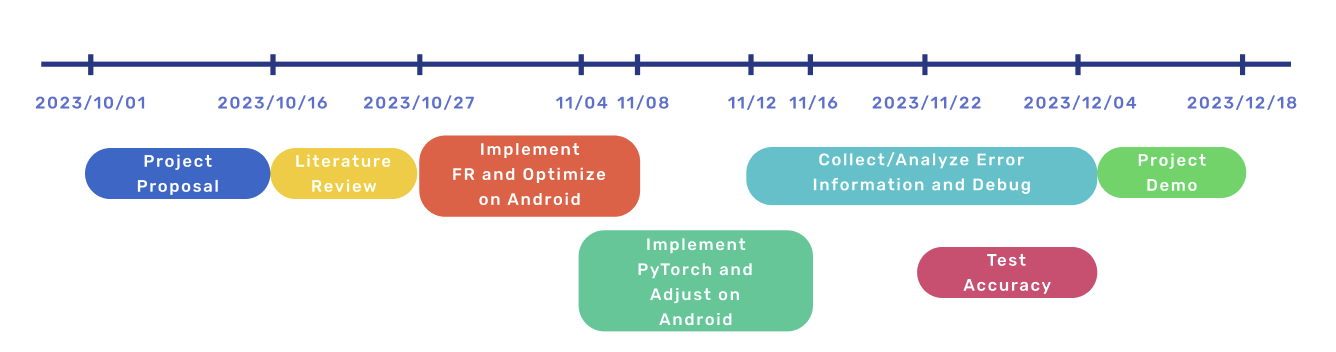
\includegraphics[width=1\textwidth]{./figure/timeline.png}
\caption{Timeline for FR implementation on Mobile Devices}
 \label{timeline_fig}
\end{figure}


\section{Short Description of 5 LABS}

In this paper, we will divide the project into five labs (milestones), which can help us to double check our progress and adjust it timely.

\begin{itemize}
	\item Deploy the Frequency Regularization algorithm with the UNet (one basic Neural Network) on the computer and adjust some parameters for the Android emulator. 
	
	\item Attempt to implement PyTorch library on the Android emulator and summarize the error messages in order to further analyze.
	
	\item Analyze the error messages and explore the methods to change PyTorch library on the Android.
	
	\item Attempt to change something on the FR algorithm to make it match the current Android system. 
	
	\item Test all functions and neural networks to check the effectiveness and accuracy on the Android system after importing the compressed neural network. We will compare the result between the computer and mobile devices. 
	
\end{itemize}

\pagebreak

\section{Literature Review}

\subsection{Review of AI Benchmark for Running Deep Neural Networks}
Nowadays, with the rapid improvements in mobile devices, they have reached the levels that can only be achieved on the previous PCs. Although there are a lot of improvements, mobile devices can still not run all the artificial intelligence applications smoothly. In the existing paper~\cite{Andrey2019Aibenchmark}, Ignatov explores further the current state of deep learning within the Android system.

In the early 1980s, digital signal processors (DSPs) started to appear in people’s view. DSPs started to appear in mobile devices (i.e. mobile phones) in the 1990s, working for voice coding and compression for the first time. The power of DSPs increased significantly as time went on. For now, the powerful DSPs can easily used for some AI and deep learning applications, such as image classifiers, facial recognition, and image style transfer. But there are still some large and complex Neural Networks such as BigGAN and StyleGAN.

In this existing paper~\cite{Andrey2019Aibenchmark},  a fabless semiconductor company, Qualcomm, introduced the Snapdragon Neural Processing Engine (SNPE) SDK, which is a powerful software development kit, including CPU, GPU, and DSP. Applying this SDK, allowed more Neural Networks to be deployed on mobile devices. Moreover, another company HiSilicon Kirin, introduced a specialized Neural Processing Unit (NPU) for fast vector and matrix-based computations commonly used in AI. In Ignatov’s research, he also mentioned other big companies like Media Tek and Samsung, which also had technology improvements for mobile devices, being good for deployment of Neural Networks on mobile devices.

AI Benchmark is just a tool or test, which is used to measure and evaluate the performance of AL algorithms on Android devices. Most researchers use this tool to determine the efficiency of the up-to-date hardware, which is manufactured by the majority of big companies. 

\subsection{Review of Neural Network Compression}

In order to learn how the four algorithms, ELM~\cite{akusok2019metal}, NestDNN~\cite{fang2018nestdnn}, “One-show Whole Network Compression”~\cite{kim2016compression}, and Frequency Regulation~\cite{zhao2023frequency} work, we have to figure out what is Neural Network. A Neural Network is a computational model, including many interconnected elements, which are inspired by the biological nervous system~\cite{picton1994neural}. The network usually has three layers: input, hidden and output layers. In a nutshell, it is an attempt to make machines simulate the way the human brain works. For the learning process of Neural Networks, the first process is always called backpropagation, adjusting the weights of the connections based on the data the model trained on. During its training process, the network just feeds data to the input layers and computes an output. Then compare the output with the expected one, adjusting the weights of the connections to minimize the possible errors.

With the increasing size of the neural network and the increasing amount of its complexity, it is quite difficult to deploy the neural network on devices, especially mobile devices with limited resources. In order to solve this problem, neural network compression was born at the right moment. The general goal of compression is to make the networks more efficient and faster. In the existing paper~\cite{neill2020overview} of the compression, we can find the common ways for compressing networks in Table~\ref{neuralcompress-table}. In our words, we can always consider the compression as a process, which converts a large and complex book to a simple and summary abstract. Moreover, the process should also retain the main content and information.

\begin{table}[htbp]
	\centering
	\caption{Four techniques involved in Neural Network Compression.}
	\label{neuralcompress-table}
	\centering
	\begin{tabular}{|p{3cm}|p{10cm}|}
		\hline
		\textbf{Techniques} & \textbf{Explaination} \\
		\hline
		Pruningl&Removing unnecessary neurons or connections.\\
		\hline
		Quantization&Reducing the precision of weights.\\
		\hline
		Knowledge Distillation&Transferring knowledge from a large model to a small one.\\
		\hline
		Tensor Decomposition&Breaking down tensors into simple forms.\\
		\hline
	\end{tabular} 
	%}
\end{table}



\subsection{Review of High-Performance Extreme Learning Machine (ELM)}
The Extreme Learning Machine is a learning algorithm for single-hidden-layer feedforward neural networks, where the weights and biases of its hidden layer are generated randomly. The existing paper~\cite{akusok2019metal}, reveals that because of this feature, ELM usually has a faster speed than other traditional neural network learning algorithms. 

Currently, ELM has become more and more important since the rise of edge computing. In Cao’s existing research~\cite{cao2020edgecomputing}, we can find that the traditional cloud computing is not the best way anymore because of large-scale data, slow response speed and poor security. Edge computing acts as an important role, in order to solving the increasing volume of data and processing demands. Since edge computing can operate in close proximity to data sources, it enables more efficient data processing. According to the characteristics of edge computing, it allows algorithms to run on mobile devices directly, providing a more convenient computing environment for users. Despite the plenty of advantages of edge computing, it still has some limitations for the implementation of high-quality Neural Network applications.

Akusok and his teammates found a new ELM implementing method, which is tailored for mobile devices with GPU acceleration. Their method combines the speed of a direct non-iterative solver with minimal memory requirements, making it suitable for edge computing situations. By comparing the performance between two different types of devices, iPad Pro and PC, it shows a result that the GPU on the iPad performs way better than the CPU on the laptop, which trained a 19000 neuron model using less than one gigabyte of memory successfully. Because of Akusok’s experiment~\cite{akusok2019metal}, tells us the potential for running Neural Networks on limited mobile devices and it also highlights the significance of the ELM.

ELM also has some limitations. As the existing paper~\cite{akusok2019metal} mentioned, first of all, ELM is sensitive to certain types of data (i.e. ill-conditioned data), making it less accurate and reliable in some special situations. It also has a tendency to overfit, which means it might perform really well on training data but not as well on unseen data. Moreover, we need to remember that there is no one-size-fits-all setting for ELM. Different situation needs to change different parameters for ELM. In our words, finding the correct settings for ELM is just like a guessing and decision game, which is not always ideal for consistent results.

\subsection{Review of NestDNN}
Currently, more and more mobile devices, like smartphones, drones, and augmented reality headsets, are trying to change our daily lives, leading to the increasing demand for mobile devices. Since our researchers want to run the Neural Networks on our own mobile devices, we find that an algorithm called NestDNN may probably solve this problem. 

For this topic, there are two main challenges that need to be solved: Multi-tenant Characteristics and Context Changes in Mobile Settings. Mobile devices often run multiple applications at the same time, and their resource availability can fluctuate because of various factors such as launching new applications or changing application priorities. This is also the main reason our own mobile devices can not support large Neural Networks since they do not have enough memory space. Here is a new algorithm NestDNN which is designed to address the dynamic nature of runtime resources in mobile vision systems. The main purpose of this is to enable resource-aware multi-tenant on-device deep learning, allowing each deep learning model to provide flexible resource-accuracy trade-offs. Through this idea, it can always select the optimal resource-accuracy trade-off for each model dynamically, making sure to utilize all the existing memories effectively and maximizing the performance of the implementation.


Fig.~\ref{nestdnn} illustrates the architecture of NestDNN, which is divided into an offline stage and an online stage. The existing paper~\cite{fang2018nestdnn} about NestDNN discussed a new model pruning and recovery scheme inside the offline stage to achieve deployment of Neural Networks on mobiles. 

To explain the detail of how NestDNN tackles the two challenges mentioned above, NestDNN utilizes a state-of-the-art \textit{Triplet Response Residual} (TRR) approach to rank the filters in a basic and unmodified deep learning model, such as Vanilla Model in Table~\ref{nest-table}. In the existing paper~\cite{fang2018nestdnn}, in order to solve context changes in mobile settings, NestDNN also explores an easy model freezing and filter growing, in order to generate the multi-capacity model in an iterative manner.	

In the existing experiment~\cite{fang2018nestdnn}, we can find that NestDNN achieves up to a 4.2\% increase in inference accuracy, doubles the video frame processing rate, and reduces energy consumption by 1.7 times. Because of this experimental result, NestDNN is indeed a useful and easy method for deploying deep learning on mobile devices.


\subsection{Review of One-shot Whole Network Compression}
There are many constraints of mobile devices, such as computing power, battery capacity, and memory capacity. Yong-Deok Kim~\cite{kim2016compression} illustrates his method to solve this problem by presenting a new scheme for compressing convolutional neural networks (CNNs).

For this topic, there is one main challenge in deploying CNNs on mobile devices: limited resources. Running some deeper CNNs, especially for complex tasks like ImageNet classification, is still hard to implement. In the existing paper written by Kim~\cite{kim2016compression}, there is a new method called “one-shot whole network compression” which is a simple and effective way to compress CNNs. This existing algorithm can be divided into three steps: rank selection with variational Bayesian matrix factorization (VBMF), Tucker decomposition on the kernel tensor, and fine-tuning to recover any loss in accuracy. Fig.~\ref{one-shot-steps} shows the scheme of these three steps of this algorithm.

%\begin{figure}[!h]
	%\centering
	%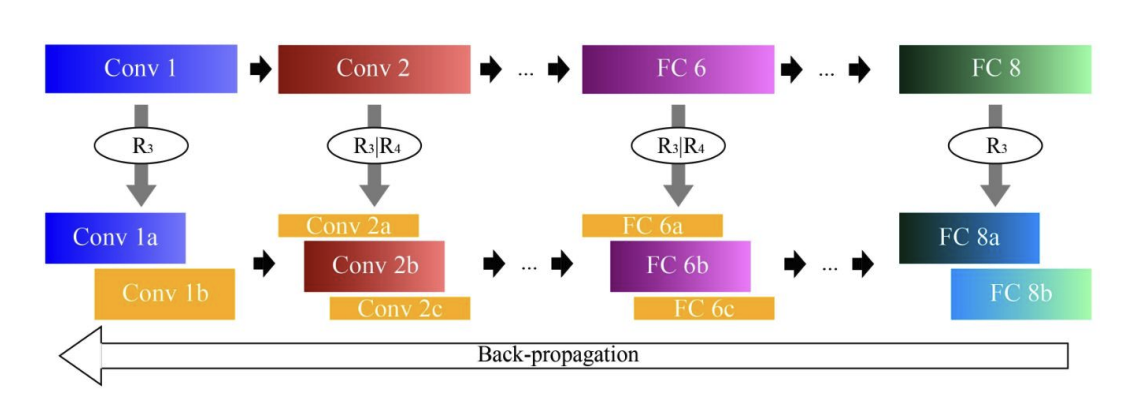
\includegraphics[width=1\textwidth]{./figure/one-shot-steps.png}
	%\caption{The scheme of one-show whole network compression, which includes three steps~\cite{kim2016compression}.}
	%\label{one-shot-steps}
%\end{figure}

In Kim’s paper~\cite{kim2016compression}, rank selection with variational Bayesian matrix factorization (VBMF) aims to determine the rank of each layer in the neural network. By applying VBMF on each kernel tensor, it can find noisy variance, rank, and rank recovery easily in an automatic way. It makes good preconditions for Tucker decomposition. Tucker decomposition on the kernel tensor is used to compress both convolutional and fully-connected layers of the neural network. It preserves the essential features, meanwhile, compressing successfully. After doing the two steps, Kim’s algorithm applies find-tuning to recover the loss in accuracy. This process makes sure that the compressed model retains its performance and accuracy close to the uncompressed model.

Since the simplicity, effectiveness, and it can compress the whole network, “One-shot Whole Network Compression” can be considered as a good algorithm. However, this algorithm has some potential limitations as well. According to the experiment in Kim’s paper, it is not fully investigated whether the rank selected is optimal or not. Moreover, it may affect the speed-up ratio since it lacks cache efficiency, in the $1 \times 1$ convolution.

\subsection{Review of Frequency Regularization}

Until now, many neural networks have been discovered or created by researchers and enhanced the features for model training. However, there exists a problem where the size of the neural networks is growing bigger. It can lead to concerns about information and storage overload because of the numerous numbers of parameters. If we want to implement the neural networks on limited hardware devices, applying some neural network compression algorithms is a method to fit the specifications. 

In most neural network research, we deduce that the network performance is because of the parameters. For instance, if we implement image segmentation, high-frequency components are not as crucial for the task since they capture the details of the image which is not necessary for the segmentation. Therefore, applying the frequency domain transform is a practical method. Also, since the frequency domain transform converts the signals into numerical data, we can easily manipulate the quantitative image information for the compression algorithm. In frequency regularization, it focuses on implementing the transform to restrict the information redundancy. The reason is because of the interpretation of the complicated architectures of the networks. Frequency domain transforms for compressing networks may not work as expected on the pre-trained models~\cite{zhao2023frequency}. 

When applying the neural network compression algorithms, we want to ensure the accuracy of the output compared with the original dataset. Although there may still exist some shortcomings of this algorithm, such as the total training time, we are still researching frequency regularization to be our target to implement neural network compression. The reason is because of the main following reasons: First, we can apply this algorithm to general neural network architectures. Second, it does not reduce the accuracy percentage. We will introduce them respectively. 

We can achieve frequency regularization by two processes. The first one is the dynamic tail truncation, and the other is the inverse discrete cosine transform (IDCT). Fig.~\ref{idct} shows the frequency regularization process. 


The dynamic tail truncation is used in this algorithm. From the research paper, the authors concluded that most parameters in convolutional networks can be eliminated. However, there exists an issue where the parameters that are not eliminated may affect the backpropagation. Therefore, the training loss may stay the same in many epochs. The strategy of dynamic tail truncation addresses this issue by continuously setting a few tail elements to 0 in every epoch but not directly setting most of them at once.

The idea behind the frequency regularization is to maintain the tensors in the frequency domain instead of the spatial domain. By implementing this, it allows the tail elements to be eliminated by a dot product with the zigzag mask matrix. After the dynamic tail truncation mentioned above, the algorithm then inputs the tensors to the inverse discrete cosine transform. The purpose of the inverse discrete cosine transforms is not only the role of reconstructing the spatial tensors. An inverse discrete cosine transform process can be implemented for tensors with any form. It leads to an important functionality, for instance, applied to any tensors from neural networks. 

\subsection{Review on Implementation on Mobile Devices}

Nowadays, mobile devices have more and more powerful hardware so that any neural network with fewer parameters can run. For instance, the Android library mentioned the pre-trained models are implementable, and we have successfully implemented them. However, in our project, we are trying to implement more advanced neural networks which may have more parameters involved. We also target to successfully apply the frequency regularization to the neural networks and implement the neural network on the mobile devices. In the following instances, some researchers successfully implemented the neural network on mobile devices. 

In Jin's paper, they implement deep convolutional neural networks on a mobile coprocessor by executing an efficient routing strategy. It is to maximize the utilization of available hardware resources. Moreover, the performance is maintained to a high standard in real-world applications. The implementation is an example of a successful case to run a neural network on mobile devices by the hardware accelerator. As mentioned in previous sections, although the processor of mobile devices has dramatically increased over decades, the real-time performance is still inferior to computers. A simple explanation of the preparation for the hardware implementation in Jin's research is to apply a memory router on their hardware compromisation. The purpose of memory routers is to process all incoming and outgoing data streams. It can also distinguish works from one or more collections. When running the algorithm, the software compiler will allocate the hardware resources to the router for processing jobs. One of the main reasons for implementing a memory router is to make the implementation more efficient. The paper states that the efficient design of the memory routing can allow the maximum utilization that leads to the result in peak performance. The idea behind the implementation is to target the efficiency and scalability of mobile platforms for deep convolutional neural network~\cite{6908370}.

In Castanyer's paper, they try to identify the most challenging part when deploying deep learning-based software in mobile applications. It includes what are the challenges that we may encounter during the implementation of the neural network on mobile devices and how we can control the complexity while maintaining a high amount of accuracy. The researchers used PyTorch and the Android framework to design some studies and set goals to diagnose the challenges. After some experiments, they discovered a few categories that needed to be considered. The first category is the challenge that is verified to be real and concerning. It includes software-data dependency, sustainability, and frameworks in the early stages. The second category is the challenge that has been identified but is not faced in the study. It includes explainability. The last category is the newly defined challenges based on their experiment studies. The researchers mainly focus on fixing the first category by applying the data augmentation technique to reduce the data-software dependency and increase the sustainability of the applications~\cite{cast2020integration}.



\small
\bibliographystyle{unsrt}
% \bibliographystyle{plain}
\bibliography{ref.bib}  




\end{document}
